% !TEX program = xelatex
\documentclass[11pt]{beamer}

\usepackage{unicode-math}
\usepackage{amsmath}
\usepackage{amsfonts}
\usepackage{amssymb}
\usepackage[style=ddmmyyyy]{datetime2}
\usepackage{graphicx}
\usepackage{hyperref}
\usepackage{fontspec}
\usepackage[dvipsnames]{xcolor}
\usepackage{tikz}
\usepackage{soul}
\usepackage{ulem}

\makeatletter
\def\input@path{{../../theme/}}
\def\beamer@shrinkfactorinv{1}
\makeatother

%beamer setup
\usetheme[subsectionpage=progressbar]{mis}
\setbeamerfont{caption}{size=\footnotesize}
\setsansfont{Lato}[Numbers=OldStyle]
\setmathfont{STIX Two Math}[Scale=MatchLowercase]
\setmonofont{Consolas}[Scale=MatchLowercase]

%tikz 
\usetikzlibrary{calc} 
\usetikzlibrary{arrows, decorations.markings, positioning, backgrounds, shapes}
\definecolor{EMP}{HTML}{77DD77} % Green1
\definecolor{NOR}{HTML}{06500C} % Green2
%tikz settings
\renewcommand{\ULdepth}{3pt}
\tikzset{
  EMP/.style={% Style for empatized boxes
      rectangle, line width=1pt,
      anchor=west,
      %underline, % new property
      align=center,
      text=Black,
      minimum height=.8cm,
      text height=1.25ex,
          text depth=.25ex,
      fill=EMP,
      draw=black,
  },
  NOR/.style={% Style for normal boxes.
      rectangle, 
      line width=1pt,
      anchor=west,
      align=left,
      minimum height=.6cm,
      text height=1.25ex,
          text depth=.25ex,
          text=white,
      fill=NOR,
      draw=black,
      inner ysep=5pt
  }
}
\def\relation(#1)#2[#3]#4{%
  \begin{scope}[shift={(#1)}] 
      \node[font=\bf, anchor=west] (Title) at (-0.25,0.75) {#3}; 
       \edef\k{0}% Variable for box positión
       \edef\x{0}% Variable for named coordinate centering - below box
       \foreach \id/\style in {#4} {%enter sub frame data Name/Boxtype ,Name2/Boxtype | An space before Boxtype is needed 
            \node[\style] (h) at (\k pt,0) {\id}; %  % Draw a node depending on the variables.
            \pgfmathparse{\k+0.5*width{"\id"}+3.4pt} % Uses the textwidth to calculate named coordinate  
            \xdef\x{\pgfmathresult} % The resul is saved in the variable \x
            \draw (\x pt,-0.4) coordinate (\id#2); %Create a named coordinate concatenated: "sub frame data Name"+"identifier"
            \pgfmathparse{\k+width{"\id"}+6.8pt}% Calculate positión for each subframe box.       
        \xdef\k{\pgfmathresult}% Save the value to be added to the next iteration value.
       }    
  \end{scope}
}

\author{Lê Thành Văn}
\title{Các dạng chuẩn của CSDL quan hệ}
\institute{Khoa Hệ thống thông tin quản lý}
\date{\today}
\hypersetup {
	colorlinks = true
}
%\usecolortheme{seahorse}
% graphic path
\graphicspath{{../../media/}}

\renewcommand{\figurename}{Hình}
\newcommand{\fd}[2]{#1 \rightarrow #2}%
%
\AtBeginSection{
  \frame{
    \sectionpage
  }
}
\begin{document}
\begin{frame}
  \titlepage
\end{frame}

\section{Giới thiệu}
\subsection{Định nghĩa}
\begin{frame}
  Chuẩn hóa cơ sở dữ liệu (csdl) là quá trình tách bảng dữ liệu nhằm:
  \begin{itemize}
    \item giảm thiểu việc dư thừa dữ liệu, và
    \item hạn chế lỗi có thể phát sinh trong quá trình thay đổi dữ liệu.
  \end{itemize}
\end{frame}

\begin{frame}
  Việc chuẩn hóa csdl dựa trên các dạng chuẩn (normal form) được Edgar F. Codd
  đề ra trong mô hình quan hệ của mình.
\end{frame}
\subsection{Các loại lỗi}
\begin{frame}
  \textbf{Lỗi khi thay đổi dữ liệu} (thêm, sửa hoặc xóa) là dạng lỗi khi dữ liệu được thay đổi không tương thích 
  với cấu trúc hoặc dữ liệu hiện có.
\end{frame}

\begin{frame}
  Giả sử thông tin giảng viên \textit{cần} bao gồm mã môn học họ giảng dạy.
  Tuy nhiên, một giảng viên mới có thể chưa có môn, dẫn đến không thể thêm thông tin của họ.

  \begin{figure}
    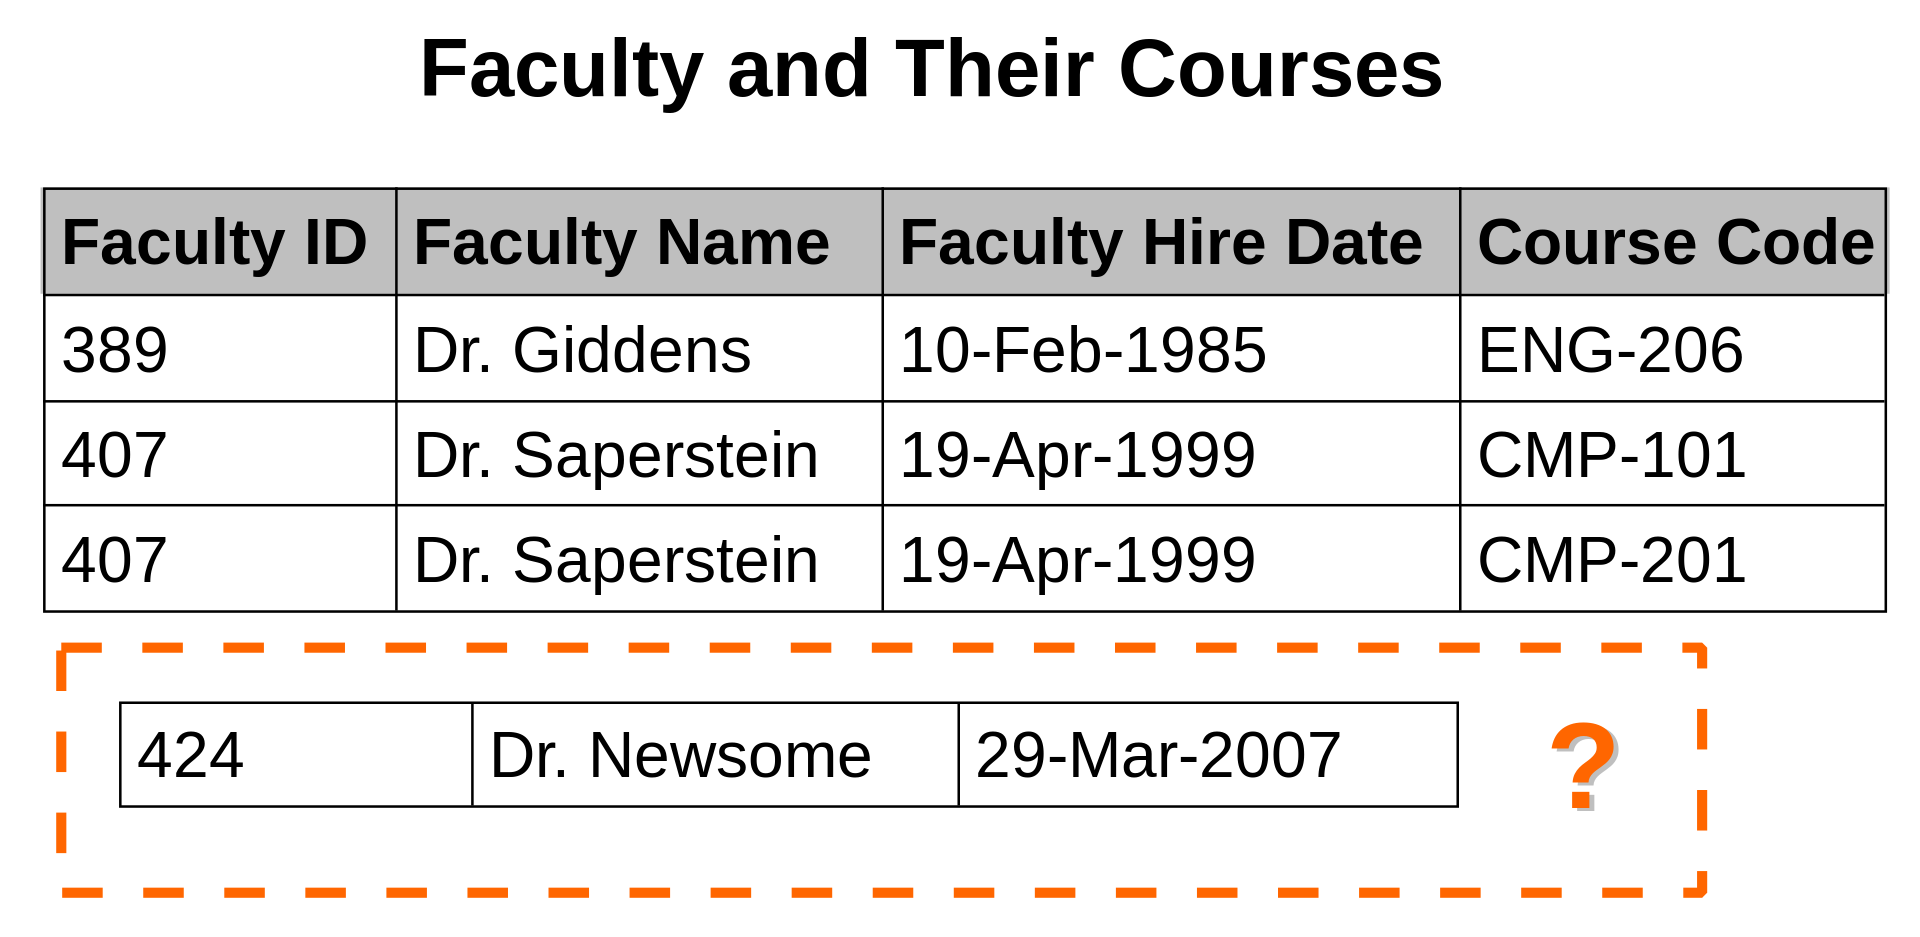
\includegraphics[width=0.75\textwidth]{COS212/ia.png}
    \caption{\textit{Lỗi khi thêm dữ liệu}}
  \end{figure}
\end{frame}

\begin{frame}
  Một thông tin có thể xuất hiện nhiều lần trong một bảng, nên khi thay đổi có thể bị sót, 
  dẫn đến thông tin không nhất quán trong csdl.
  \begin{figure}
    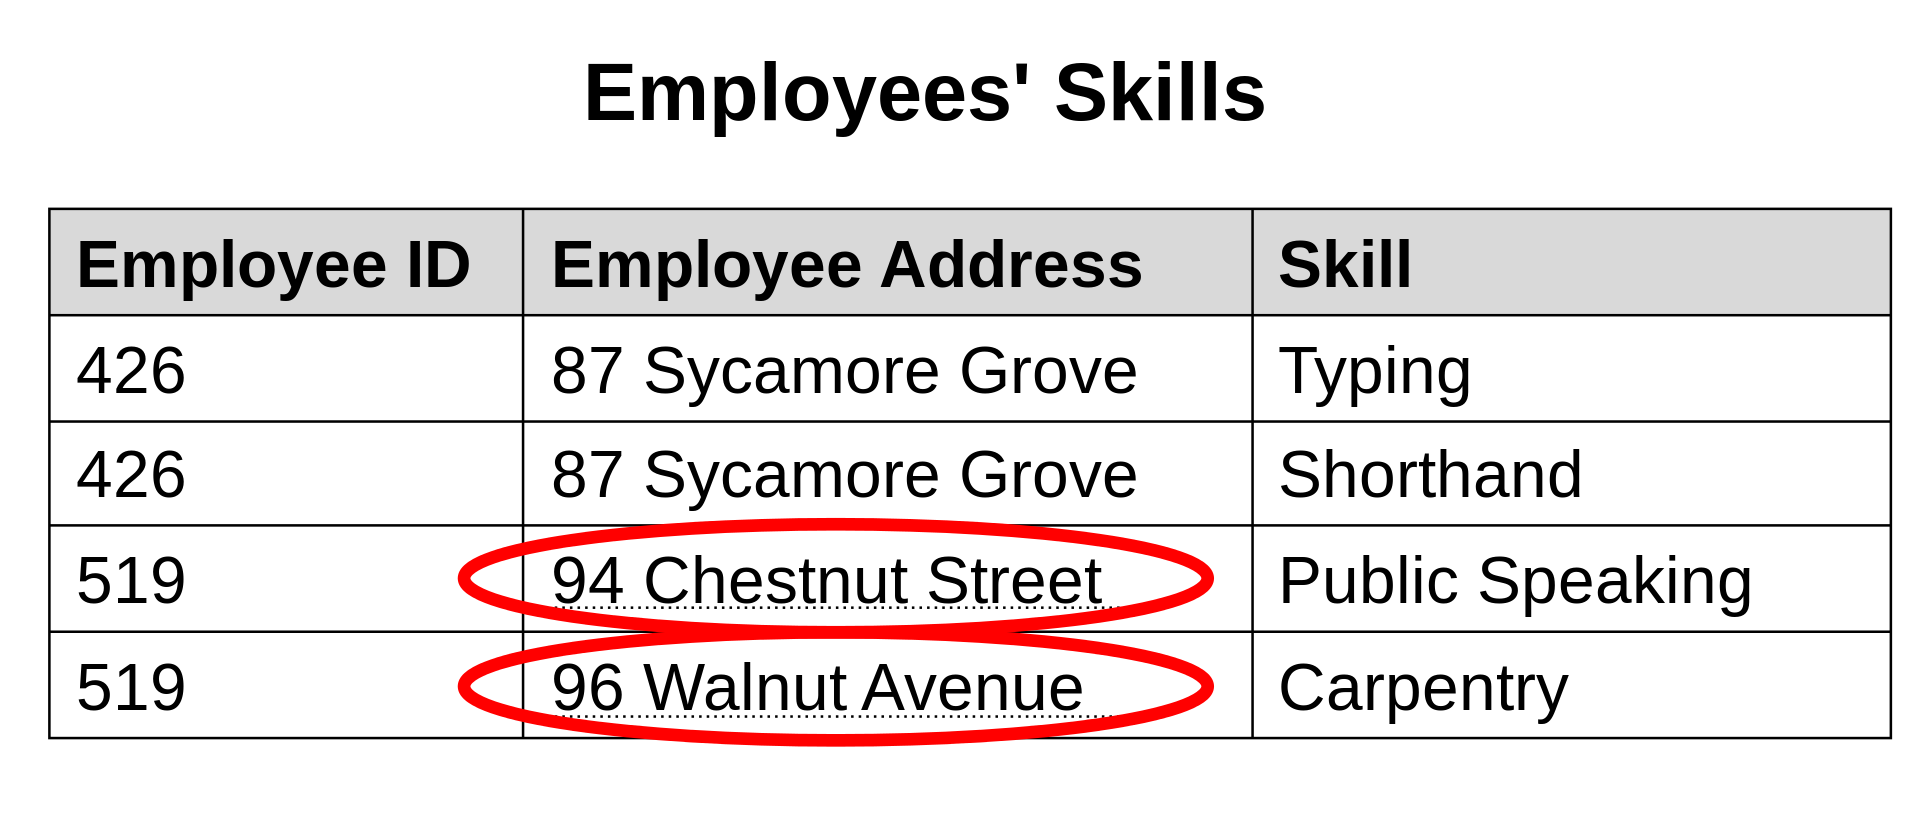
\includegraphics[width=0.75\textwidth]{COS212/ua.png}
    \caption{\textit{Lỗi khi sửa dữ liệu}}
  \end{figure}
\end{frame}

\begin{frame}
  Lỗi khi xóa dữ liệu là dạng lỗi mà khi xóa một thông tin này có thể xóa những 
  thông tin (không cần xóa) khác.
  \begin{figure}
    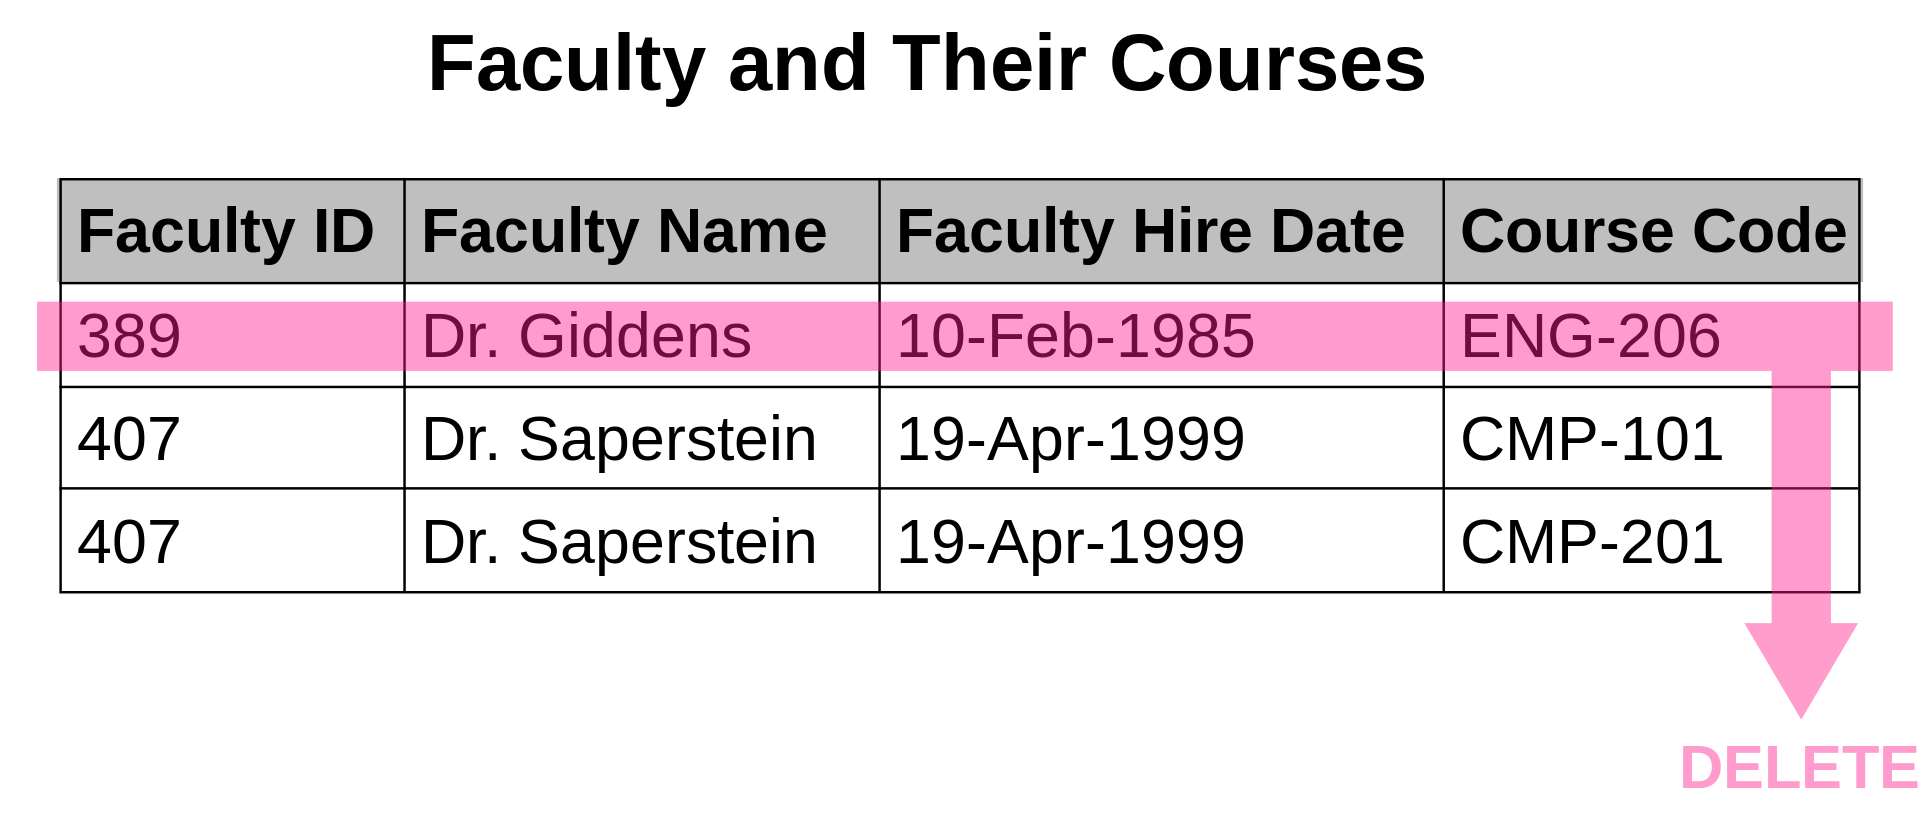
\includegraphics[width=0.75\textwidth]{COS212/da.png}
    \caption{\textit{Lỗi khi xóa dữ liệu}}
  \end{figure}
\end{frame}

\subsection{Các dạng chuẩn}
\begin{frame}
  Các dạng chuẩn thường gặp bao gồm (từ thấp đến cao):
  \begin{itemize}
    \item Dạng chuẩn 1 (First Normal Form, 1NF).
    \item Dạng chuẩn 2 (Second Normal Form, 2NF).
    \item Dạng chuẩn 3 (Third Normal Form, 3NF).
    \item Dạng chuẩn Boyce-Codd (Boyce-Codd Normal Form, BCNF, 3.5NF). 
  \end{itemize}
\end{frame}

\begin{frame}
  Việc đạt được một dạng chuẩn cao có nghĩa là phải thỏa mãn điều kiện của các dạng chuẩn thấp hơn nó.\\
  Tức là, không thể đạt được dạng chuẩn 3 nếu như không đạt được dạng chuẩn 1 hoặc dạng chuẩn 2.
\end{frame}

\begin{frame}
  Một csdl quan hệ được gọi là \textbf{đã chuẩn hóa} nếu như nó đạt được dạng chuẩn 3.
\end{frame}

\section{Các dạng chuẩn}
\begin{frame}
  Chúng ta sẽ dùng dữ liệu sau đây để tìm hiểu về các dạng chuẩn cũng như quá trình chuẩn hóa csdl.
  \begin{figure}
    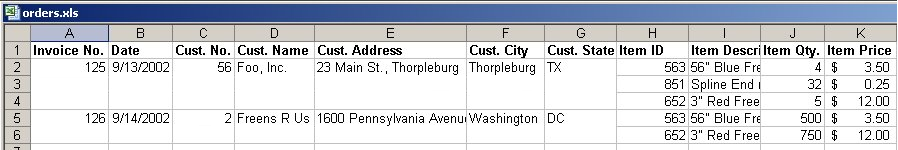
\includegraphics[width=\textwidth]{COS212/un.png}
    \caption{\textit{CSDL chưa chuẩn hóa}}
  \end{figure}
\end{frame}

\subsection{Dạng chuẩn 1}
\begin{frame}
  \textbf{Dạng chuẩn 1} đạt được khi giá trị của mỗi ô là nguyên tố, tức là
  không thể chia nhỏ giá trị đó thành nhiều phần có ý nghĩa tương đương.
\end{frame}

\begin{frame}
  Để đưa cơ sở dữ liệu về dạng chuẩn 1, chúng ta cần tách các giá trị không nguyên tố 
  thành từng dòng riêng biệt.
  \begin{figure}
    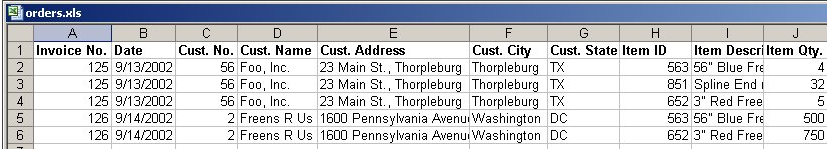
\includegraphics[width=\textwidth]{COS212/1nf.png}
    \caption{\textit{CSDL đạt dạng chuẩn 1}}
  \end{figure}
\end{frame}

\begin{frame}
  Hoặc là cũng có thể tách các giá trị không nguyên tố thành bảng riêng,
  kèm với một khóa ngoại tham chiếu đến bảng cũ.
  \begin{tikzpicture}
    \relation(0, 0){1}[INVOICE]{
      InvNo/EMP,
      Date/NOR,
      CusNo/NOR,
      CusName/NOR,
      CusAddr/NOR,
      CusCity/NOR,
    }
    \relation(0, -2.5){2}[INVOICE-ITEM]{
      ItemId/EMP,
      InvNo/EMP,
      ItemDesc/NOR,
      ItemQuan/NOR,
      ItemPrice/NOR,
    }
    \draw[thick,->,thick,>=latex]
    (InvNo2)++(0.1,0) -- ++(0,-.5) -- ++(-2.5, 0) -- (InvNo1)++(-.5, -.5);
  \end{tikzpicture}
\end{frame}
\subsection{Phụ thuộc hàm}
\begin{frame}
  Để hiểu về dạng chuẩn 2, chúng ta cần đến khái niệm phụ thuộc hàm.\\
  \textit{Định nghĩa}. Cho quan hệ $R(X, Y, ...)$, ta nói $Y$ phụ thuộc vào $X$ nếu như
  khi biết được giá trị của $X$ thì ta xác định được giá trị duy nhất của $Y$. \\
  Ký hiệu: $X \rightarrow Y$, đọc là $X$ xác định $Y$ hoặc $Y$ phụ thuộc vào $X$.  
\end{frame}

\begin{frame}
  \begin{columns}
    \begin{column}{0.5\textwidth}
      Với dữ liệu ở bảng bên, ta có thể thấy các phụ thuộc hàm sau:
      \begin{itemize}
        \item<1-> $\fd{A}{B}$, $\fd{A}{C}$, \dots
        \item<2-> $\fd{BC}{A}$, $\fd{BC}{DE}$
        \item<3-> \dots
      \end{itemize}
    \end{column}
    \begin{column}{0.5\textwidth}
      \begin{tabular}{|c|c|c|c|c|}
        \hline
        \textbf{A} & \textbf{B} & \textbf{C} & \textbf{D} & \textbf{E} \\
        \hline
        a1 & b1 & c1 & d1 & e1 \\
        \hline
        a2 & b1 & c2 & d2 & e1 \\
        \hline
        a3 & b2 & c1 & d1 & e1 \\
        \hline
        a4 & b2 & c2 & d2 & e1 \\
        \hline
        a5 & b3 & c3 & d1 & e1 \\
        \hline
      \end{tabular}
    \end{column}
  \end{columns}
\end{frame}

\begin{frame}
  Cho quan hệ $R(X, Y, Z)$, phụ thuộc hàm có một số tính chất:
  \begin{itemize}
    \item \textbf{Tính phản xạ}. $\fd{XY}{X}$.
    \item \textbf{Tính tăng trưởng}. Nếu $\fd{X}{Y}$ thì $\fd{XZ}{YZ}$.
    \item \textbf{Tính bắc cầu}. Nếu $\fd{X}{Y}$ và $\fd{Y}{Z}$ thì $\fd{X}{Z}$.
  \end{itemize}
  \textbf{Câu hỏi}. Chứng minh nếu $\fd{X}{Y}$ và $\fd{X}{Z}$ thì $\fd{X}{YZ}$.
\end{frame}

\begin{frame}
  
\end{frame}
\subsection{Dạng chuẩn 2}
\begin{frame}
  \textbf{Dạng chuẩn 2} đạt được khi:
  \begin{itemize}
    \item Đạt được dạng chuẩn 1.
    \item Không tồn tại phụ thuộc hàm một phần trong csdl.
  \end{itemize}
\end{frame}
\end{document}